\chapter{Planning Algorithm}
\section{Introduction}

\todo{Mention that ego vehicle, model car, robot are used interchangeably in the document}

The goal of the path planner is to navigate the robot from the start configuration to destination by blending in the traffic. Path planning module is dependent on various modules to receive the data regarding the perceived environment and invoke a set of modules to move the robot safely. It has to drive the robot ahead considering the traffic rules, obstacles, kinematic and dynamic constraints of the robot and not compromising on the safety and comfort of the passengers inside. The main aim of this chapter is to derive path planning techniques to drive the robot safely to destination.

This section is organised to provide an overview of different modules needed for path planning and methods used in each module to achieve the goal. Path planning starts from the initial understanding of where the ego vehicle is and where to go, subsection \ref{localization} describes regarding localization of ego vehicle to provide this data, subsection \ref{route_planner} provides the information on how a global path to the destination is calculated. An autonomous vehicle should have the understanding of surroundings in terms of where other vehicles are, where pedestrians are, traffic signal information etc., Prediction module described in \ref{prediction} details further on how the ego vehicle perceives environment. The next subsection \ref{motion_planner} describes further in-depth details about the short term planning algorithm or the trajectory planner. The final module in the discussion is control unit, described in subsection \ref{traj_follower}. It is responsible for translating the path in space-time into steering and acceleration values to drive the robot.

Figure \ref{path_planner} represents the general architecture of the planning module. It details on the flow of information, dependencies, relative execution frequency. All the modules are implemented as independent nodes in Robot Operating System(ROS) and communicate with each other using ROS messages.
\begin{figure}[h]
    \centering
    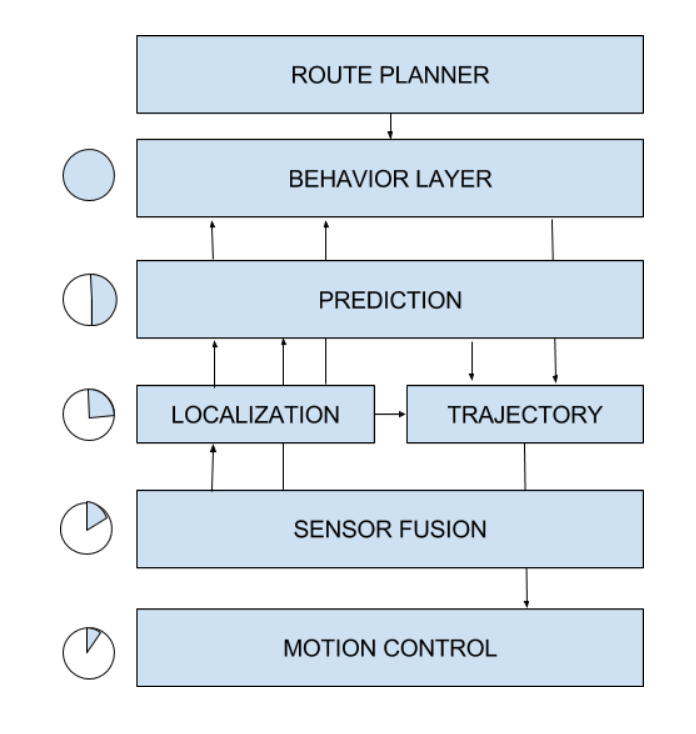
\includegraphics[width=0.8\textwidth]{Images/path_planner.png}
    \caption{Path Planning Module}
    \label{path_planner}
\end{figure}
\todo{Add reference as udacity course material for path planning overview picture,
add different color to highlight the main modules I am working on}

\section{Localization} \label{localization}

Localization module is responsible for providing the current state of the vehicle in terms of position, orientation, speed(linear and angular) and acceleration. The localization module implemented on the modelcar has two sub components Vehicle Odometry and Global Position estimation using Visual GPS. Odometry is calculated with dead reckoning \cite{dead_reckoning} with speed information from motor and yaw information from Inertial Measurement Unit(IMU). The localization module combines odometry with the information received from a visual GPS node(tracks markers on roof) to correctly estimate the state of the ego vehicle. 

\section{Prediction} \label{prediction}

Prediction and Sensor fusion modules receive the data from various sensors such as Cameras, LIDAR etc and fuse them together to create an environment model, classify objects into different categories and predict the state of obstacles in the surroundings. Due to time constraints this thesis simulates a prediction module to provide motion planner with obstacle information in different traffic scenarios.

\section{Route Planner} \label{route_planner}
Route Planner is responsible for finding a global route between the vehicle current state and the goal state based on the static characteristics of the environment/map such as lane information, speed limits etc. Route planner obtains this information generally from the maps or other formats to represent the road network. In this thesis a simple model called " Road Navigation Definition File(RNDF)"  \cite{rndf_darpa} \cite{rndf_fu} is used to represent the route network. Next subsections details further about RNDF and how global reference route is calculated.

\subsection{RNDF}

This chapter details about the RNDF file \cite{rndf_darpa} that defines the road network(set of roads/ areas connected together) over which the vehicle can traverse. This representation of road is developed by DARPA for its Autonomous Vehicles Urban Grand Challenge. RNDF representation first divides the traversable areas into two parts, segments and free zones and mentions regarding connections across these areas. Free zones represent areas such as parking lots and road segments are drivable lanes. Each segment has multiple lanes, each lane has way points along the driving direction. More significant information about way points such as whether it is a stop sign etc can be added. Each segment/zone is connected to one another using exits, they represent the connections between one segment way points at start/end to another. Figures \ref{rndf_segment} \ref{rndf_exits} \ref{zone_segment} \cite{rndf_darpa} represent various portions of the route representation and Figure \ref{map_rndf} details regarding one of the route network of map used in Lab experiments. 

\begin{figure}
    \centering
    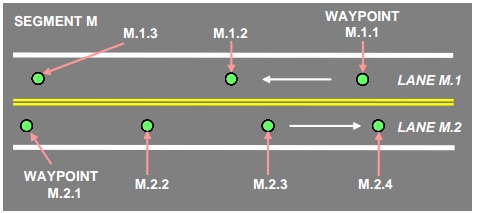
\includegraphics[width=0.8\textwidth]{Images/rndf_segment.png}
    \caption{Segment representation in RNDF - Segement M has two lanes M1, M2 and each lane has way points 1-N}
    \label{rndf_segment}
\end{figure}

\begin{figure}
    \centering
    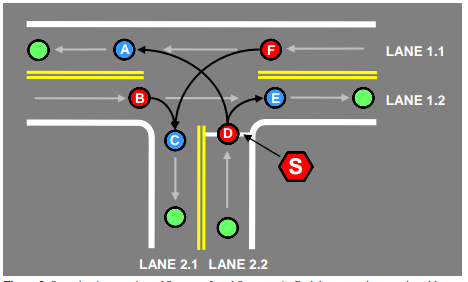
\includegraphics[width=0.8\textwidth]{Images/rndf_exits.png}
    \caption{Exit representation in RNDF - Connections between two segments in a T-Junction}
    \label{rndf_exits}
\end{figure}

\begin{figure}
    \centering
    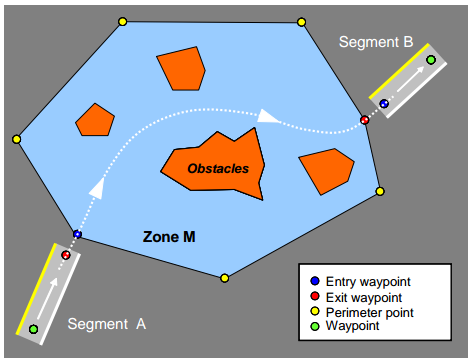
\includegraphics[width=0.8\textwidth]{Images/zone_segment.png}
    \caption{Zone Representation in RNDF - Connection between Segments and Zone}
    \label{zone_segment}
\end{figure}


\begin{figure}
    \centering
    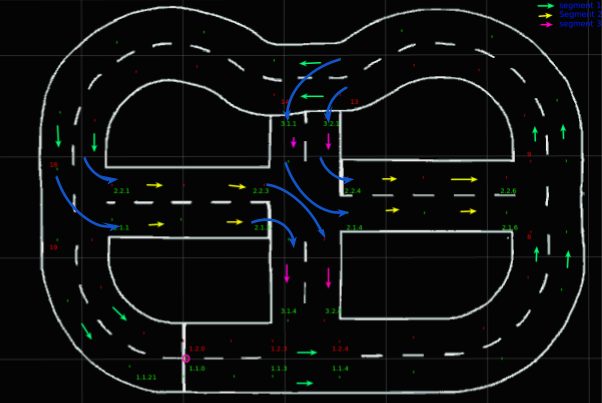
\includegraphics[width=0.8\textwidth]{Images/map_rndf.png}
    \caption{Road network for the map used to test model Car}
    \label{map_rndf}
\end{figure}

\todo{foot note - source of images}
\todo{Add Appendix for how to create the RNDF file for model car}


\subsection{Path Representation and calculation}

The data in RNDF is represented in the form of a tree with connections across way-points which in turn are related to their parent objects lanes and segments. The global path from source to destination is the shortest path between the closest way-point to ego vehicles current position and closest way-point to the destination in graph. Then the shortest path found is sub divided into sub-paths based on which segment the way points lie. A sub-path represents a set of way points in one segment, once the ego vehicle is at the end of one sub-path it receives a notification from the trajectory planner that a goal has been reached, then the route planner transmits the next sub path to the trajectory planner, this process is repeated till destination is reached. Figure \ref{path_Segmentation} details further about the division of shortest path across different segments. This method also reduces the memory needed in modeling the road in trajectory planning stage.

\begin{figure}[H]
    \centering
    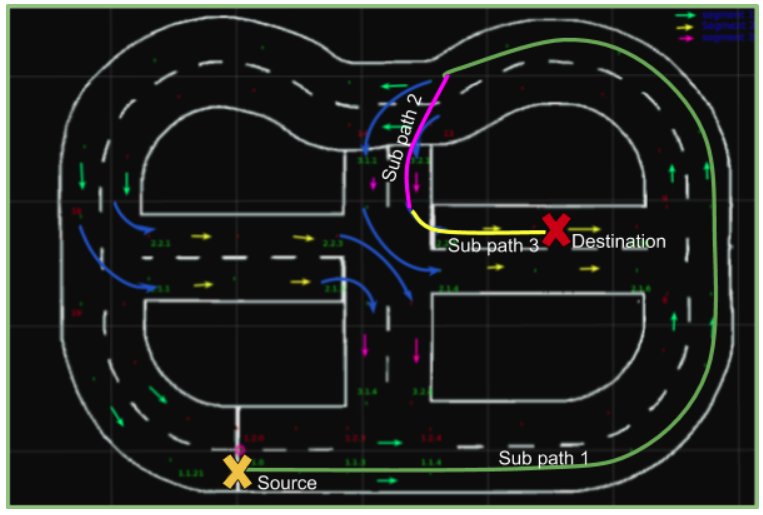
\includegraphics[width=0.8\textwidth]{Images/path_Segmentation.png}
    \caption{Division of shortest path in road network into Sub paths across different segments}
    \label{path_Segmentation}
\end{figure}

\subsection{Behavioral Layer}
\todo{check if this should be moved to related work}
Behaviour layer plays an important role in making path planning, it is responsible for understanding the scenario and makes decisions according to various traffic rules, constraints and choices that will make driving more efficient for the vehicle. One such decision example is which lane the vehicle should drive, the decision is made by understanding whether the lane is empty for a significant time, if the ego vehicle is about to take an exit then a right lane is preferred, lane based on driving speed etc. Behavioural layer is a huge research topic in itself and not in the scope of this thesis, currently, a simple simulated approach is implemented where the user can provide inputs to decide behaviour using mouse clicks etc.

\section{Motion Planner} \label{motion_planner}

This section discusses the planning algorithm to create short-term trajectories in accordance with the global path to reach destination. The subsection \ref{timing_constraints} provides an overview of the timing Horizon and constraints in dynamic environments for different modules in planning. The next subsection \ref{frenet_frame} details regarding path modeling and how this will improve the efficiency of planning along with constraints. It also discusses on approximation method used to convert coordinates from Cartesian to Frenet frame. The core of this chapter is creation of trajectories which is discussed in detail in subsection \ref{traj_creation}. The next sections \ref{osbtacle_check_satic} and \ref{obstacle_check_dynamic} explain further on how the created trajectories are evaluated for collision with static and dynamic obstacles. Next subsection \ref{traj_Selection} details on how a final trajectory is selected from the set of evaluated trajectories for the trajectory follower to follow.

\subsection{Temporal Horizon} \label{timing_constraints}
Time is an important aspect for planning in dynamic environments and there are several timing variables associated with planning. This section is mainly adopted from the doctoral thesis \cite{eth_timing_constraints}. These timing parameters define how far into the future different sub modules of planning will be valid. 
 \todo{ check if this name is needed and add footnote to link "Autonomous vehicle navigation in dynamic urban environments for increased traffic safety" of Macek kristijan doctoral work} 

The initial timing variable in motion planning is timing horizon $ T_m $. It is measure of how far into the future trajectory of the ego vehicle is planned. Second is the prediction horizon $ T_p $, it is measure of how far into the future the motion of dynamic obstacles around can be predicted. The fundamental requirement of planning to be valid is that $ T_m  \le  T_p $ such that planning is done only so far into the future as the environment is predictable. 

Thirdly $ T_d $ indicates the computation time of the motion plan. Assuming planning is done in cycles, the plan created in previous cycle is executed in current cycle, thus $ T_d  \le  T_m $. If this condition fails then the planner will run out of path for the next cycle. In general $ T_d \ll T_m $. $ T_s $ is the perception update cycle time, i.e., perception module updates the state of surrounding dynamic obstacles every $ T_s $ seconds. In general world the predicted trajectories for duration $ T_p $ will not hold true as the behavior of these vehicles is not controlled by the ego vehicle. Thus the constraint $ T_s  \le T_p $ should be valid. This creates an uncertainty in modeling of the environment, thus the execution duration of current plan $ T_e $ beyond $ T_s $ is not sensible. This is due to fact that obstacle trajectories may have changed in $ T_s $ and executing the old trajectory may lead to collisions invalidating the trajectory created for $ T_m $. 

\todo{check if it is needed to write on time discretization}

The next timing constraint in consideration is $ T_e $, control execution time of the current plan. $ T_e $ should not exceed the perception update time $ T_s $. This restriction also imposes additional constraint on $ T_d $ (motion plan computation time), $ T_d \le T_e $. 

In summary, timing constraints described above identify the relation between different modules such as motion planning, motion prediction and execution. It is also important to predict farther into future than $T_s$ or  $T_e$ for completeness of motion planner with respect to goal objective, uncertainty also increases with time. In general a farsighted uncertain motion plan potentially directing the vehicle towards goal is better, but this plan needs to be re-evaluated and re-executed in short intervals for correctness. 

\todo{check if this should be moved to implementation}
In general behaviour of other vehicles can be predicted for up-to 5s probabilistically, thus the temporal $ T_m $ \& prediction $ T_p $ horizon are chosen to be 5s. The planner has an execution time $ T_d $ far less than 100ms on a low power computational hardware which allows a high update rate allowing lower values for $ T_e $. As obstacle detection is simulated a pessimistic value of 250ms for $ T_s $ is chosen and even higher update frequency can be chosen as the planner is fast enough to react. 

\todo{time to see minimum distance ahead with current speed, minimum time to bring car to halt at good speed etc etc. }

\subsection{Path Modelling} \label{frenet_frame}

 Planned global path is in Cartesian coordinate system, one of the problems with the Cartesian coordinate system is that the due to variation in curvature local planning becomes complex. To address this issue planning in curvilinear system or Frenet Frame or  lane adoptive (SL) coordinate system has been adopted by researchers, \cite{traj_planner_optimization} \cite{spatio_temporal_state_lattice} \cite{diss_shui_phd_thesis} \cite{real_time_traj_plan_article} \cite{volvo_reactive_traj} \cite{curvilinear_System_Automated_Drv} are some of the research works in which Frenet frame is adopted. In this method center of the lane/road or preplanned global path is used as reference longitudinal coordinate(S) and perpendicular distance with respect to the lane center is considered as lateral coordinate(L/D) as represented in Figure \ref{sl_over_xy} \cite{diss_shui_phd_thesis}.  Thus once converted, (S,L) coordinate system essentially is a straight road.
 
 \begin{figure}[H]
    \centering
    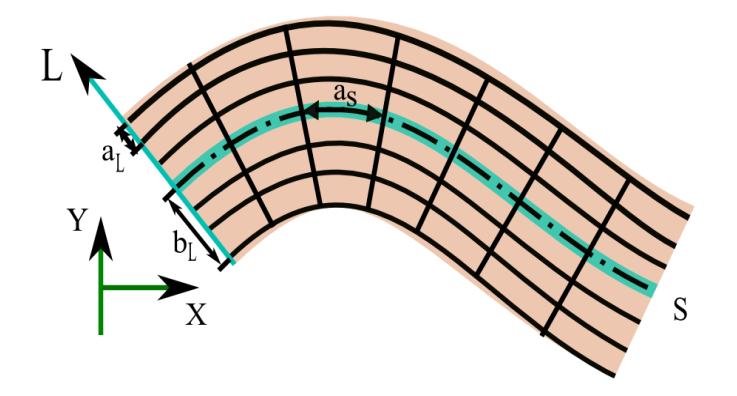
\includegraphics[width=0.8\textwidth]{Images/sl_over_xy.png}
    \caption{SL coordinate system laid over XY coordinate system}
    \label{sl_over_xy}
\end{figure}
\todo{add diss shui reference in foot note}
 
 Conversion from Frenet frame to Cartesian and vice versa is a widely researched topic and many techniques exist which offer different level of complexity and accuracy. In this thesis an approximation method is used to convert between these two coordinate systems similar to \cite{volvo_reactive_traj}. This method is computationally inexpensive and provides required level of accuracy for modelcar. To convert an xy coordinate to SL coordinate, (x,y) is projected onto the current path represented by different way points as in figure \ref{xy_sl_conversion}, cumulative distance till this point gives the S coordinate and the perpendicular distance between the projected point and the current point provides the L coordinate. A similar process is used to convert S,L coordinate to x,y coordinate. S is used to find a point on a segment represented by way points, a point at a perpendicular distance L gives the x,y coordinate. We assume that the path between two way points is linear which reduces the computational complexity in approximation. This approximation how ever approaches zero error when the spacing between two way points approaches zero. Adding dense way points in the curves significantly reduces the approximation error. There are different methods discussed in \cite{lengthparameterized} \cite{Wangrobustand} which provide better accuracy in calculating the paths. 
 
 As observed in Figure \ref{sl_over_xy}, in SL coordinate system the size of the unit distance is not constant, it stretches in the convex side of road and gets compresses in concave side of the reference line. This is especially an issue in curves with lower radius of curvature, this will affect the velocity planning thus causing discomfort in some cases. There is a wide research in topic of velocity and path smoothening which counter these affects.
 
 In summary, curvilinear coordinate system makes planning easier but needs extra computation in conversion from one format to other. It also introduces errors and inefficiencies in planning if the complete planning is done in SL coordinate system.
 
 \begin{figure}[H]
    \centering
    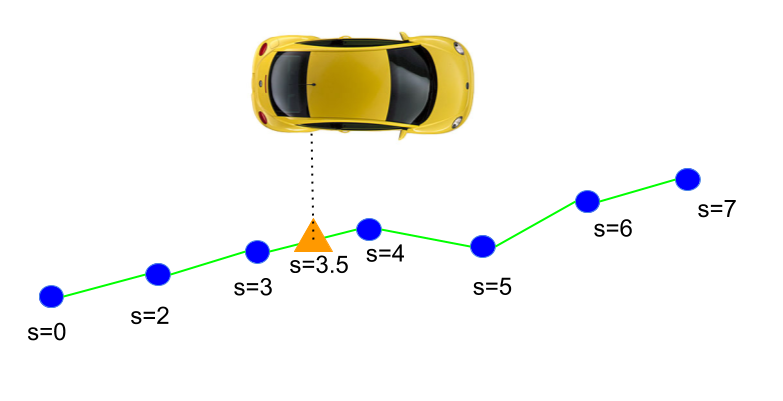
\includegraphics[width=0.8\textwidth]{Images/xy_sl_conversion.png}
    \caption{Showing projection of the current position of the car shown by green triangle to s coordinate system. Each circle represents a node, and the lines between them are links.}
    \label{xy_sl_conversion}
\end{figure}
\todo{add VOLVO reference reference in foot note and also remove the orange dots}


\subsection{ Trajectory Creation} \label{traj_creation}

The core of this thesis is the trajectory planner that drives the robot from source to destination. Understanding from the behavior of human drivers in structured environments(road networks) it is necessary for the planner to create trajectories that  avoid collisions, align with the road network, smooth, continuous and comfortable. Chapter \ref{related_work} discusses a great amount of literature in motion planning techniques.

\todo{ motion planning techniques be presented properly in related work} 
%\cite{motion_planning_techniques}. 

%The approach of this thesis to create trajectories is inspired from \cite{unit_A_star} which proposes a trajectory planning technique combining path and velocity planning.

The approach proposed in this thesis is inspired by how human drive, i.e., the driver tries to maintain an optimal speed, next shift laterally based on obstacles ahead and brake if a collision is predicted with current driving state or perform an evasive maneuver. To reach a speed vehicle need to accelerate/decelerate, this can be achieved with various levels of values based on current state as, each acceleration/deceleration level chosen will result in different final states. The initial step is to sample this set of acceleration values, Figure \ref{accelerations} shows how a vehicle which approached acceleration A3 at time $t_0$ can continue to different levels of accelerations from A1 to A8. Generally, A1 represents an acceleration of around $2m^{-1}$ and A8 of up to $-8m^{-1}$ which are on the higher end of decelerations which not most of the cars are capable of performing. Generally deceleration values are up to $-4.5m^{-1}$ \cite{denmark_breaking} \cite{accelerations_study} \cite{accelerations_study_2}. Applying each of this acceleration profile to current ego vehicle state for planning horizon $ T_m $ leads to different final states of ego vehicle. The final sates will have different final velocity as shown in Figure \ref{velocities}, different distances traversed as in Figure \todo{create distances travelled picture from simulator}.

Change of acceleration is defined as jerk and to create smooth trajectories it is important that the trajectories generated by the motion planner must have least jerk. There are various techniques to create these Jerk free trajectories as discussed in chapter \ref{related_work}. The selection of smoothness depends also on the capabilities of the ego vehicle and controller to track these fine trajectories.
 
 \begin{figure}[H]
    \centering
    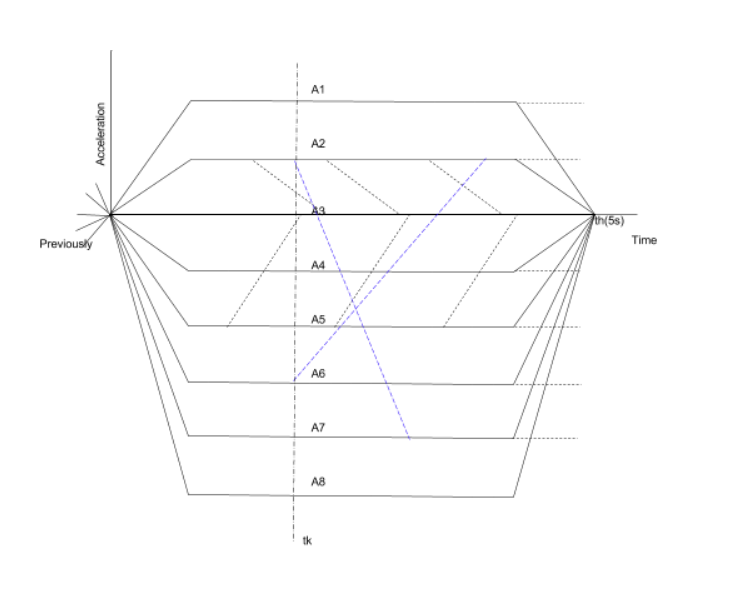
\includegraphics[width=0.8\textwidth]{Images/accelerations.png}
    \caption{Different acceleration profiles a car can follow from current state.}
    \label{accelerations}
\end{figure}

 \begin{figure}[H]
    \centering
    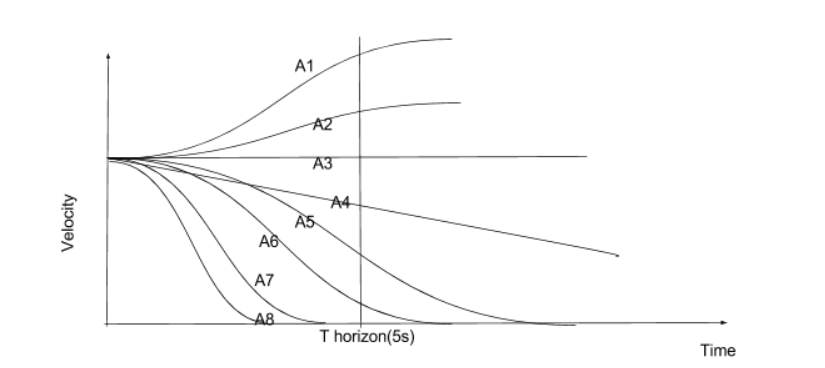
\includegraphics[width=0.8\textwidth]{Images/velcoities.png}
    \caption{Different acceleration profiles a car can follow from current state.}
    \label{velocities}
\end{figure}

\todo{Redraw these profiles neatly with proper labels - acc and velocity}

Acceleration profiles discussed above solve the problem of longitudinal planning but to avoid obstacles the ego vehicle should also plan lateral(sideways) shifts in its trajectory. Similar to different accelerations, lateral shifts are sampled and combined along with acceleration samples to create final states. Lateral shifts can be mapped either as a function of time or distance traversed by ego vehicle. The research of Werling et al. \cite{werling_frenet} suggests that at lower speeds it is advantageous to map lateral shift as a function of distance and at higher speed as a function of time. As this thesis is intended towards urban environments with limited speeds, lateral shift is mapped as a function of distance traversed. Lateral shift planning in this thesis is adopted from \cite{real_time_traj_plan_article}, which uses cubic splines and models lateral shift as a parameter of longitudinal distance as shown in equation \ref{lat_shift_one}. 

\begin{equation}
l(s) = c_0 + c_1s + c_2s^2 + c_3s^3
\label{lat_shift_one}
\end{equation}

The first and second derivative of the equation \ref{lat_shift_one} are equations for lateral velocity \ref{lat_vel} and acceleration \ref{lat_acc}.

\begin{equation}
    \frac{dl}{ds} = c_1 + 2c_2s + 3c_3s^2
\label{lat_vel}
\end{equation}


\begin{equation}
    \frac{d^2l}{d^2s} = 2c_2 + 6c_3s.
\label{lat_acc}    
\end{equation}

Form the boundary conditions(0- initial state, f - final state), we have

\begin{equation}
l(s_0) = l_0 , l(s_f ) = l_f
\label{lat_boudary}
\end{equation}

The angle between the road frame and the vehicle is defines as $\theta(s)$, it can be derived from the first derivative of the lateral shift with respect to s. 

\begin{equation}
\theta(s) = arctan(\frac{dl}{ds})
\label{lat_veh_theta}
\end{equation}

To ensure the generated path follows current curvature and orientation of car and the final orientation is parallel to the road segment, following conditions should be satisfied.


\begin{equation}
\theta(s_0) = \theta_0 , \theta(s_f) = 0
\label{th_bundary}
\end{equation}

The figure \ref{lat_planning} indicates how the initial orientation will affect the shape of the trajectory. 

 \begin{figure}[H]
    \centering
    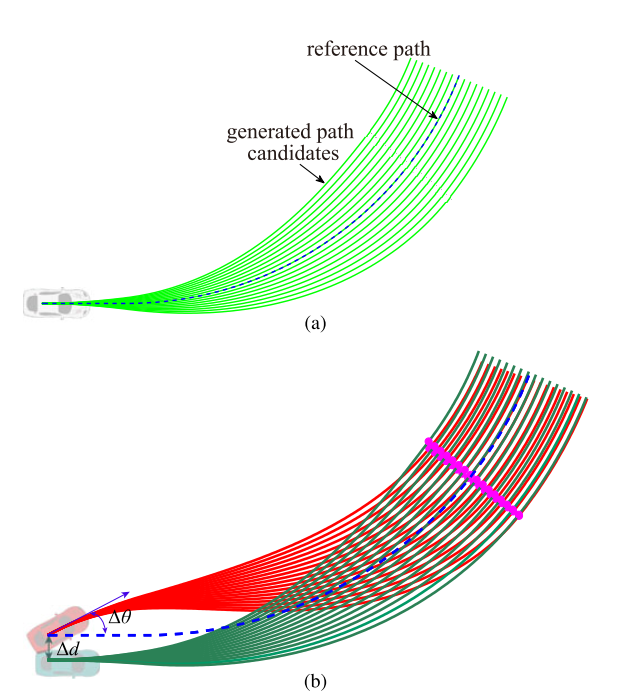
\includegraphics[width=0.8\textwidth]{Images/lateral_planning.png}
    \caption{Path candidates generation results. (a) $l_0 = 0$ and $\theta_0 = 0$ (b) $ 
l_0 = \Delta_d$ and $ \theta_0 = \Delta\theta$.}
    \label{lat_planning}
\end{figure}

\todo{create own figure}


The constants $ { c_0,c_1,c_2,c_3}  $ in equation \ref{lat_shift_one} can be obtained by solving equations \ref{lat_vel} to \ref{th_bundary}.

In summary, combining samples in acceleration and lateral shifts, multiple trajectories with different final states are created over the time horizon. In the next sections how these trajectories are tested for collision with respect to other dynamic obstacles is discussed. 

\todo{add a picture of how this will look in the end - various trajectories in planning}


\subsection{Checking for Static Obstacles} \label{osbtacle_check_satic}
The main objective of the motion planner is to derive a path that is collision free. The generated trajectories must be evaluated for collision or driving close to obstacles. There are various techniques for collision detection as discussed in the background study. This thesis developed a simple two step collision checking technique for static obstacles. A road parallel model in Frenet frame is employed for collision checking ignoring the orientation of obstacles with respect to road as described in \cite{cmu_parallel_thesis}. Using a road parallel method and dilating the obstacle for safety reduces computational complexity. 

\todo{check if all things described in road parallel model for collision checking should be discussed here}

In the first step of collision checking, obstacle coordinates are transformed into Frenet frame and represented by a length and width parallel to road. In second step, the trajectory in consideration is checked if it has a collision in longitudinal dimension(s coordinate) for length of the obstacle. As shown in Figure \ref{static_check} trajectories T0,T1 intersect in S for obstacle O1 and not for obstacle O2. The next step is to find this intersection region, I1 to I2 in Figure \ref{static_check}, the values are dilated for safety. In final it is checked whether from I1 to I2 there is a collision in lateral dimension(d) for trajectory and obstacle. This is computed by checking if at any point between I1 and I2, the lateral distance between trajectory and obstacle must always be greater than safety value as described in \ref{static_obst_safety_dist}. 

\begin{equation}
    |d\textsubscript{ego} - d\textsubscript{obst}| > car\_width/2 + obstacle\_width/2 + safety\_margin
    \label{static_obst_safety_dist}
\end{equation}
\todo{represent the parameters in terms of $d_e , c_w, o_w$ etc}

It is clearly representative from figure \ref{static_check} that the trajectory T1 has collision and trajectory T0 has no collision. Different costs can be added based on how close the ego vehicle is with respect tot he static obstacle. As per trajectory creation lateral shift changes in only one direction thus it is sufficient to check for the collision at start, end and middle of the intersected path. 


 \begin{figure}[H]
    \centering
    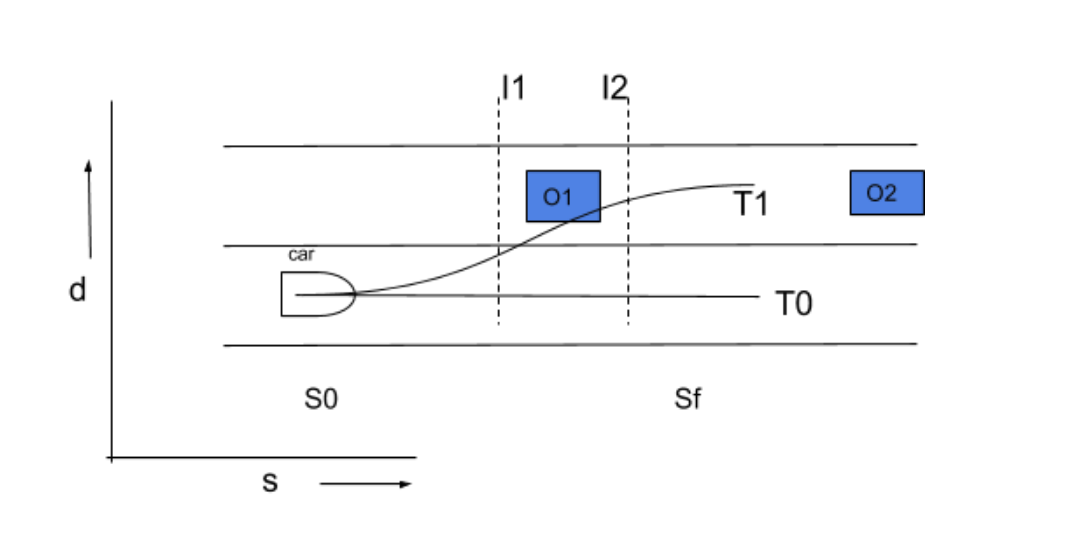
\includegraphics[width=0.8\textwidth]{Images/static_check.png}
    \caption{Collision check for static obstacles}
    \label{static_check}
\end{figure}



\subsection{Checking for Dynamic Obstacles} \label{obstacle_check_dynamic}

In dynamic environments such as cities it is key to plan trajectories predicting the position of other obstacles and not colliding into them. Predicting the future behavior of obstacles
is a challenging part in urban driving, some of the existing approaches assume dynamic obstacles as quasi-static, some assume obstacles to continue in their current detected heading, in contrast this thesis models dynamic obstacles as squares continuing with their current speed in their detected lane for planning duration similar to \ref{unit_A_star} or moving in opposite direction in lane or moving across the lane based on angle between the obstacle and road. This assumption can be justified by the fact that the trajectories are re-evaluated at high frequencies and any changes in obstacles lateral distance will be evaluated in next cycle thus keeping the vehicle safe from collision. 

The collision check for dynamic obstacles has one extra check in time over checking for static obstacles. In step one the intersection in S coordinate for obstacle and ego vehicle is found, here the length of obstacle is dilated over the distance traveled by obstacle as represented by dotted line ahead of obstacle in figure \ref{dynamic_check}. Then if the collision in S dimension exists, then the collision between ego vehicle and obstacle in lateral dimension(d) in the intersection region I1 to I2 is tested in similar way to static obstacle collision check. If the collision in d dimension exists then the s dimension where there is collision in lateral dimension(d) is found, represented with J1-J2 in figure \ref{dynamic_check} (generally this will be shorter than I1 - I2). For the range J1-J2 it is checked if they collide in time also i.e., if they reach the same location in same time, buffer of time is added to be safe. As per instructions for safe driving it is required for the car to maintain a minimum time gap 2s with the vehicle ahead. There are more formal methods \cite{mobile_eye_safety_distance} on safety distances for self driving cars. This thesis implements simple 2s rule to safety and this is a tunable parameter which can be used to increase driving aggression. Sub Figure d of \ref{dynamic_time_check} indicates the collision in time dimension for scenario presented in Figure \ref{dynamic_check}.

To check collision in time dimension, time gap between the ego vehicle and the obstacle at the S dimension intersection borders is checked as shown in figure \ref{dynamic_time_check}. If the gap is greater than 2 seconds all times and doesn't change sign then there is no collision, Figure \ref{dynamic_time_check} a) presents a situation where the obstacles get close but does not collide. Extra costs are added if the ego vehicle gets too close to obstacle. A collision occurs when the sign of time gap between the ego vehicle and the obstacle changes as shown in sub figure b and c of \ref{dynamic_time_check}. Figure e of \ref{dynamic_time_check} shows the collision when obstacle is moving in opposite direction. 

If a dynamic obstacle is found moving laterally across the road then it is represented as a static obstacle occupying the length of the road. Thus if there is a pedestrian crossing the road, trajectory is considered to be in collision if there is a collision in s dimension and there will anyways by collision in d dimension due to dilation of the pedestrian width to width of the road and no time dimension is checked.

\todo{write why simulating over time and checking for collision is not a good idea - how computational complexity increases}


\todo{Remove these pictures and add further pictures with evaluation for obstacles in same lane and opposite lane.}

 \begin{figure}[H]
    \centering
    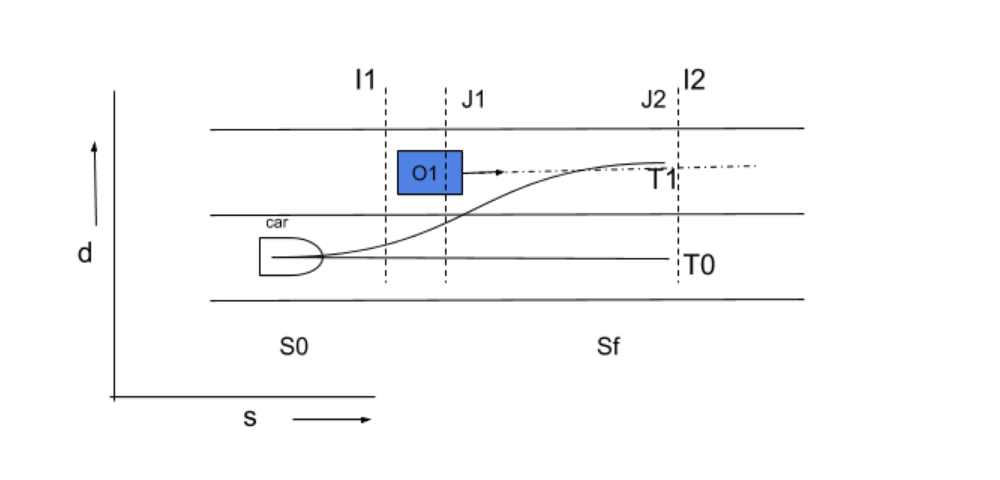
\includegraphics[width=0.8\textwidth]{Images/dynamic_check.png}
    \caption{Collision check for Dynamic obstacles}
    \label{dynamic_check}
\end{figure}

\todo{add reference to Daniel Thesis for forbidden regions etc}


\begin{figure}[h]
    \centering
    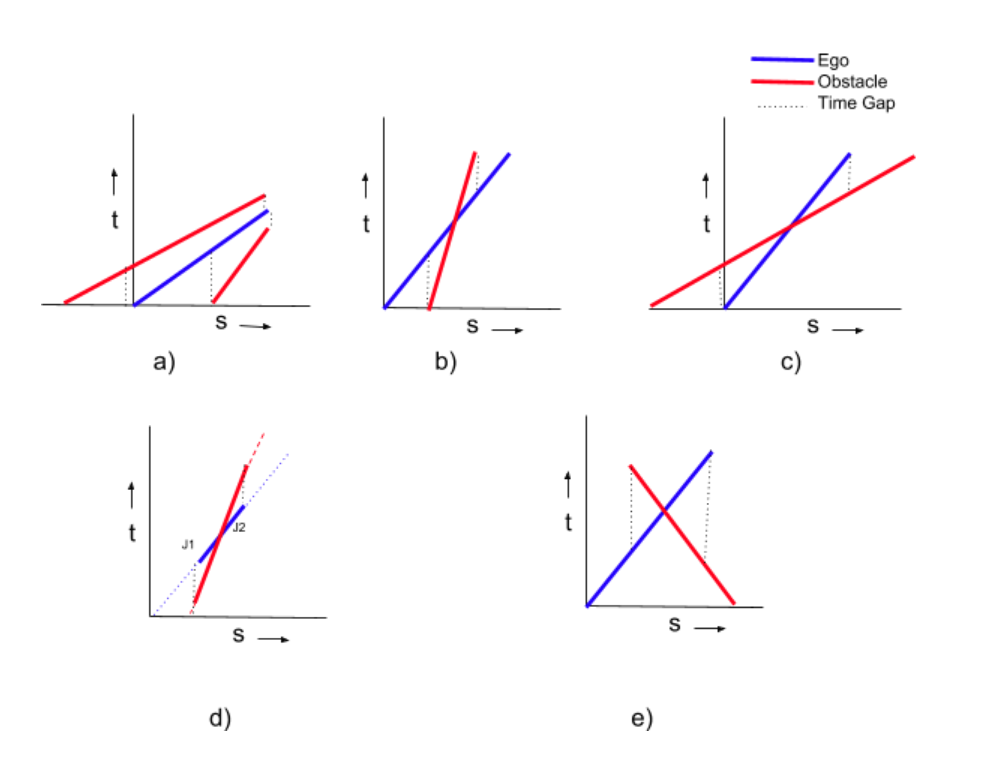
\includegraphics[width=0.8\textwidth]{Images/dynamic_Check_time.png}
    \caption{Collision check in space Time a) indicates obstacles getting close to the ego vehicle but not colliding. b) Ego vehicle hits the slow moving obstacle ahead. c) Ego vehicle is hit by fast moving obstacle behind - Situation during unchecked lane change by ego vehicle }
    \label{dynamic_time_check}
\end{figure}



%Dynamic obstacles are assumed to continue in the lane they are detected and if an obstacle is found across two lanes then it is assumed to be performing lane change and modelled as two dynamic obstacles moving straight in both lanes to overcome uncertainty.


%The collision check dynamic obstacles is performed in two stages, in first stages bounding boxes are drawn across the length of the trajectory of both the ego vehicle and the dynamic obstacle across time T. If the bounding boxes intersect then the second stage of collision check is invoked. In this step, both the dynamic obstacle and ego vehicle are moved in unit steps of time and checked for collision. As per the earlier assumption, dynamic obstacles tend to move in the lane they are detected thus to make the collision check simple, 3 lines are drawn across the corners and centre of the vehicle. The lines are extended for unit time and if the 3 lines intersect with the ego vehicle bounding square then there is a collision. The figure \ref{dynamic_obstacle} details further about the collision check.
%\todo{(The representation is not correct in figure, take the representation from the cited pages for further ease)}
%\todo{bounding boxes - Autonomous Driving in Dynamic Environments}
%\todo{Cite this paper for $3$ line collision-  An RRT-based Navigation Approach for Mobile Robots and Automated Vehicles-RRT*\_. pdf}




\subsection{Cost Functions and Trajectory Selection} \label{traj_Selection}
Selection of final trajectory is based on the different costs associated with it, costs can be static and dynamic. Static costs are known prior to trajectory creation and dynamic costs are known after the trajectory is created and evaluated. There is a wide research on different costs involved in trajectory selection as discussed in section \todo{add link to sub chapter costs in related works}

This thesis implements a simple cost function as represented in \ref{cost_eqn}, explicit smoothness costs are not considered as the target validation platform is a model car with no humans inside and limitations of model car to track a fine trajectory. 
\begin{equation}
cost = |V_a - V_t| + |a_t| + | (d_t - d_e)*k1 | + | (d_p - d_e)*k2 |\
\label{cost_eqn}
\end{equation}
$V_a$ - velocity achieved by trajectory.
$V_t$ - Target Velocity.
$a_t$ - Target Acceleration.
$d_t$ - Target lateral distance.
$d_e$ - Trajectory lateral distance.
$d_p$ - Previous target lateral for trajectory.
$k_1,k_2$ - Factors to adjust weights, currently used at 0.8 and 0.2

The Velocity and acceleration terms in cost function \ref{cost_eqn} promote higher accelerations if the target and current velocity difference is higher and lower accelerations if the difference is low. The next lateral terms promote the trajectories that are closer to the target lateral distance and also closer to the previous selection thus limiting the shifts in path selection and maintaining continuity. 

Initially all the sampled trajectories are assigned the costs based on the cost function \ref{cost_eqn} and sorted, then the trajectory with the lowest cost is evaluated for collisions first. The list is sorted again and evaluated till the top of the list has lowest cost and the trajectory is evaluated. 

\subsection{Velocity Planning}
Velocity planning is an important aspect of the planer, in general behavioral layer defines the target velocity based on speed regulation, other traffic participants, required behavior, road condition etc. In this thesis a simple approach of velocity limiting is used based on road curvature to limit lateral accelerations. Max velocity  V\textsubscript{max} is calculated based on the equation \ref{max_vel}. 

\begin{equation}
    V\textsubscript{max} = min(\sqrt{Acc\textsubscript{MaxLat} / |k(s)|} , V\textsubscript{limit})
\label{max_vel}
\end{equation}
$V\textsubscript{limit}$ - Velocity limit mentioned in road network,
$Acc\textsubscript{MaxLat}$ - Maximum Lateral acceleration(based on comfort and vehicle dynamics),
$k(s)$ - Road curvature.

\section{Trajectory Follower} \label{traj_follower}

Check whether to refer to MIG trajectory controller or write in short about the controller. 
